\documentclass{standalone}

\usepackage{tikz}
\author{George}
\title{An ArM System Sketch}

\begin{document}
\maketitle

This is a sketch for discussion.

\begin{figure}
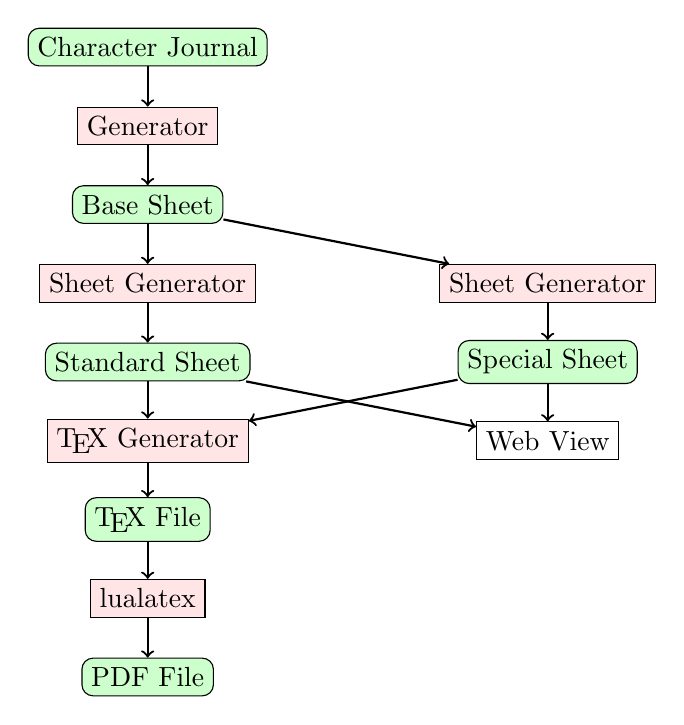
\begin{tikzpicture}
   \tikzstyle{file}=[fill=green!20,rounded corners,draw]
   \tikzstyle{transform}=[fill=red!10,draw]
   \tikzstyle{arrow}=[thick,draw,->]
   \node (cj) [file] {Character Journal} ;
   \node (gen) [transform,below of=cj] {Generator} ;
   \node (base) [file,below of=gen] {Base Sheet} ;
   \node (sgen) [transform,below of=base] {Sheet Generator} ;
   \node (sheet) [file,below of=sgen] {Standard Sheet} ;
   \node (sgen2) [transform,right of=sgen,node distance=2in] {Sheet Generator} ;
   \node (sheet2) [file,below of=sgen2] {Special Sheet} ;
   \path [arrow] (cj) -> (gen) ;
   \path [arrow] (gen) -> (base) ;
   \path [arrow] (base) -> (sgen) ;
   \path [arrow] (base) -> (sgen2) ;
   \path [arrow] (sgen) -> (sheet) ;
   \path [arrow] (sgen2) -> (sheet2) ;
   \node (tgen) [transform,below of=sheet] {\TeX\ Generator} ;
   \path [arrow] (sheet) -> (tgen) ;
   \path [arrow] (sheet2) -> (tgen) ;
   \node (tgen) [transform,below of=sheet] {\TeX\ Generator} ;
   \node (tex) [file,below of=tgen] {\TeX\ File} ;
   \node (luatex) [transform,below of=tex] {lualatex} ;
   \node (pdf) [file,below of=luatex] {PDF File} ;
   \path [arrow] (tgen) -- (tex) ;
   \path [arrow] (tex) -- (luatex) ;
   \path [arrow] (luatex) -- (pdf) ;
   \node (web) [draw,right of=tgen,node distance=2in] {Web View} ;
   \path [arrow] (sheet) -> (web) ;
   \path [arrow] (sheet2) -> (web) ;
\end{tikzpicture}
   \caption{System flow, with files in green and transformation in red.}
\end{figure}

\begin{itemize}
        \item 
File formats could be either JSON-LD, (custom) JSON, or any RDF
serialisation.
        \item 
           Only the Journal file should be edited.
        \item 
           The diagrams is shown in terms of files, but this does not
           have to imply files on disk.  They could be files transmitted
           between micro-services and clients over the network, or
           data structures within one monolithic system.
        \item 
           The system will depend on additional resource files;
           most importantly canon trait descriptions, possibly also
           other rulesets.  It is an open question what should be
           hard coded and what should be defined in customisable files.
\end{itemize}



\end{document}
